\documentclass[11pt]{article}

% Packages
\usepackage[margin=1in]{geometry}
\usepackage{amsmath, amssymb}
\usepackage{graphicx}
\usepackage{caption}
\usepackage{subcaption}
\usepackage{enumitem}
\usepackage{hyperref}
\usepackage{fancyhdr}
\usepackage{titlesec}

% Header/Footer
\pagestyle{fancy}
\fancyhf{}
\rhead{ML Project Report}
\lhead{Your Name}
\cfoot{\thepage}

% Section formatting
\titleformat{\section}{\large\bfseries}{\thesection}{1em}{}
\titleformat{\subsection}{\normalsize\bfseries}{\thesubsection}{1em}{}

% Title
\title{\textbf{Machine Learning Project Report}}
\author{Your Name \\
Course Name – University \\
\texttt{your.email@university.edu}}
\date{\today}

\begin{document}

\maketitle

\section{Task Overview}
Briefly describe the dataset or model you worked on, the goal of the project, and why the task is challenging. For example, challenges may include complex preprocessing, large dataset size, class imbalance, poor performance of baseline approaches, or the need for more complex models to achieve good results.

\section{Methods}
Explain the methods you implemented or analyzed. Include relevant equations:

\[
\min_{\mathbf{w}} \quad \frac{1}{2} \|\mathbf{w}\|^2 + C \sum_{i=1}^n \xi_i
\]

Mention any design decisions or implementation notes.

\section{Experiments and Results}
Present your results. Use figures, tables, and metrics:

\begin{figure}[h]
    \centering
    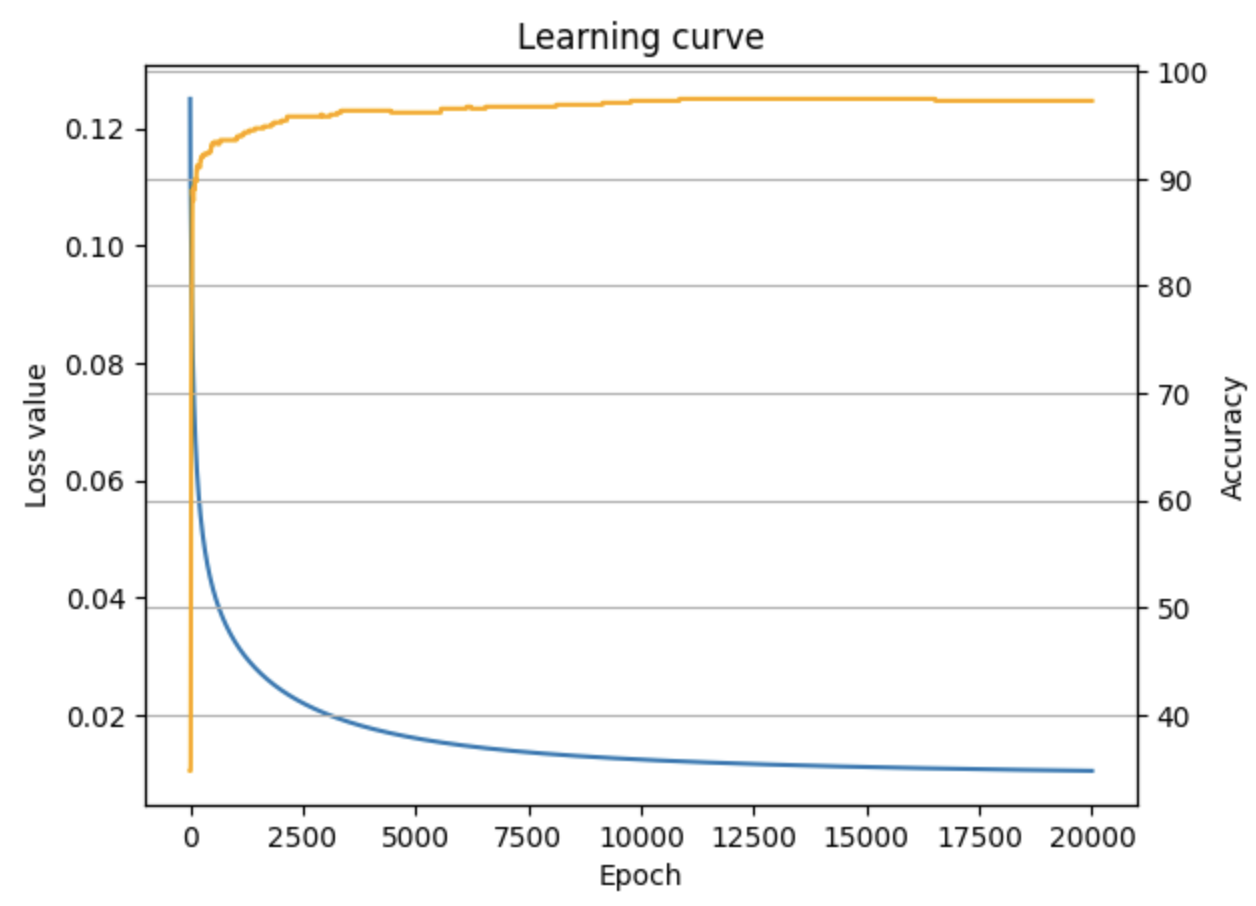
\includegraphics[width=0.5\textwidth]{ML_Project_Report_Template/figures/accuracy_curve.png}
    \caption{Training/validation accuracy over epochs.}
\end{figure}

\section{Discussion}
Summarize key findings, insights, or issues. Optionally, suggest future work or limitations.

\end{document}
